% Made up for the tikra benchmark.
\usetikzlibrary{datavisualization.formats.functions}
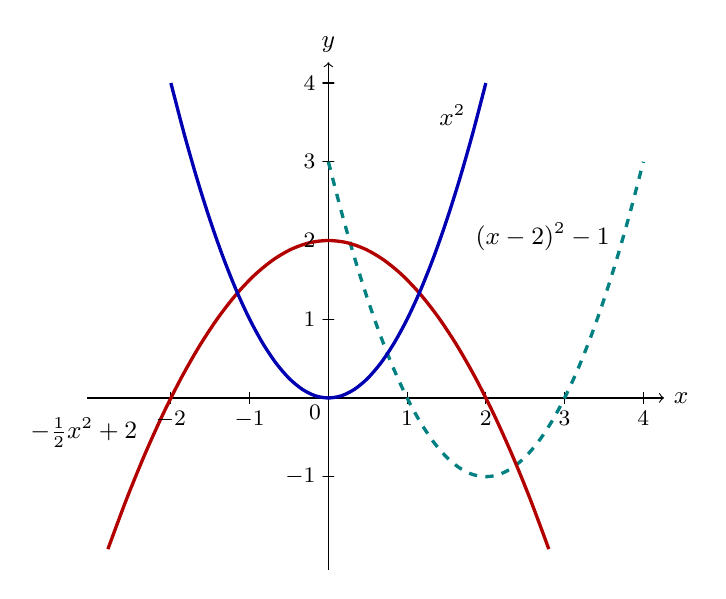
\begin{tikzpicture}
  \datavisualization [school book axes={unit=1},
      x axis={label=$x$}, y axis={label=$y$},
      visualize as smooth line/.list={up, down, shifted},
      up={style={blue!70!black, very thick}, label in data={text=$x^2$, when=x is 1.8}},
      down={style={red!70!black, very thick}, label in data={text=$-\frac12x^2+2$, when=x is -2.4}},
      shifted={style={teal, very thick, dashed}, label in data={text=$(x-2)^2-1$, when=x is 3.5}}]
    data [set=up, format=function] {
      var x : interval [-2:2];
      func y = \value x * \value x;
    }
    data [set=down, format=function] {
      var x : interval [-2.8:2.8];
      func y = 2 - 0.5 * \value x * \value x;
    }
    data [set=shifted, format=function] {
      var x : interval [0:4];
      func y = (\value x - 2)^2 - 1;
    };
\end{tikzpicture}
